\documentclass{beamer}

\mode<presentation>
{
  \usetheme{Berlin}
  \usecolortheme{default}
  \setbeamercovered{transparent}
}

\usepackage[english]{babel}
\usepackage[all]{xy}
\usepackage[latin1]{inputenc}

\usepackage{times}
\usepackage[T1]{fontenc}
\usepackage{verbatim}
\usepackage{hyperref}

\title[Sensor Fusion on a mini Unmanned Vehicle]
{Sensor Fusion on a mini Unmanned Vehicle}

\subtitle{Integrating vision-based algorithms on an Parrot AR.Drone to autonomously follow linear shaped structures in a landscape.}

\author[Verschoor ] % (optional, use only with lots of authors)
{C.~R.~Verschoor}

\institute[University of Amsterdam] % (optional, but mostly needed)
{
  Faculty of Science (FNWI) \\
  University of Amsterdam
}

\AtBeginSection[]
{
  \begin{frame}<beamer>{Outline}
    \tableofcontents[currentsection]
  \end{frame}
}

\begin{document}

\begin{frame}[plain]
\begin{center}
\Large Sensor Fusion on a mini Unmanned Vehicle
\normalsize Integrating vision-based algorithms on an Parrot AR.Drone to autonomously follow linear shaped structures in a landscape.\\\vspace{0.3cm}\small
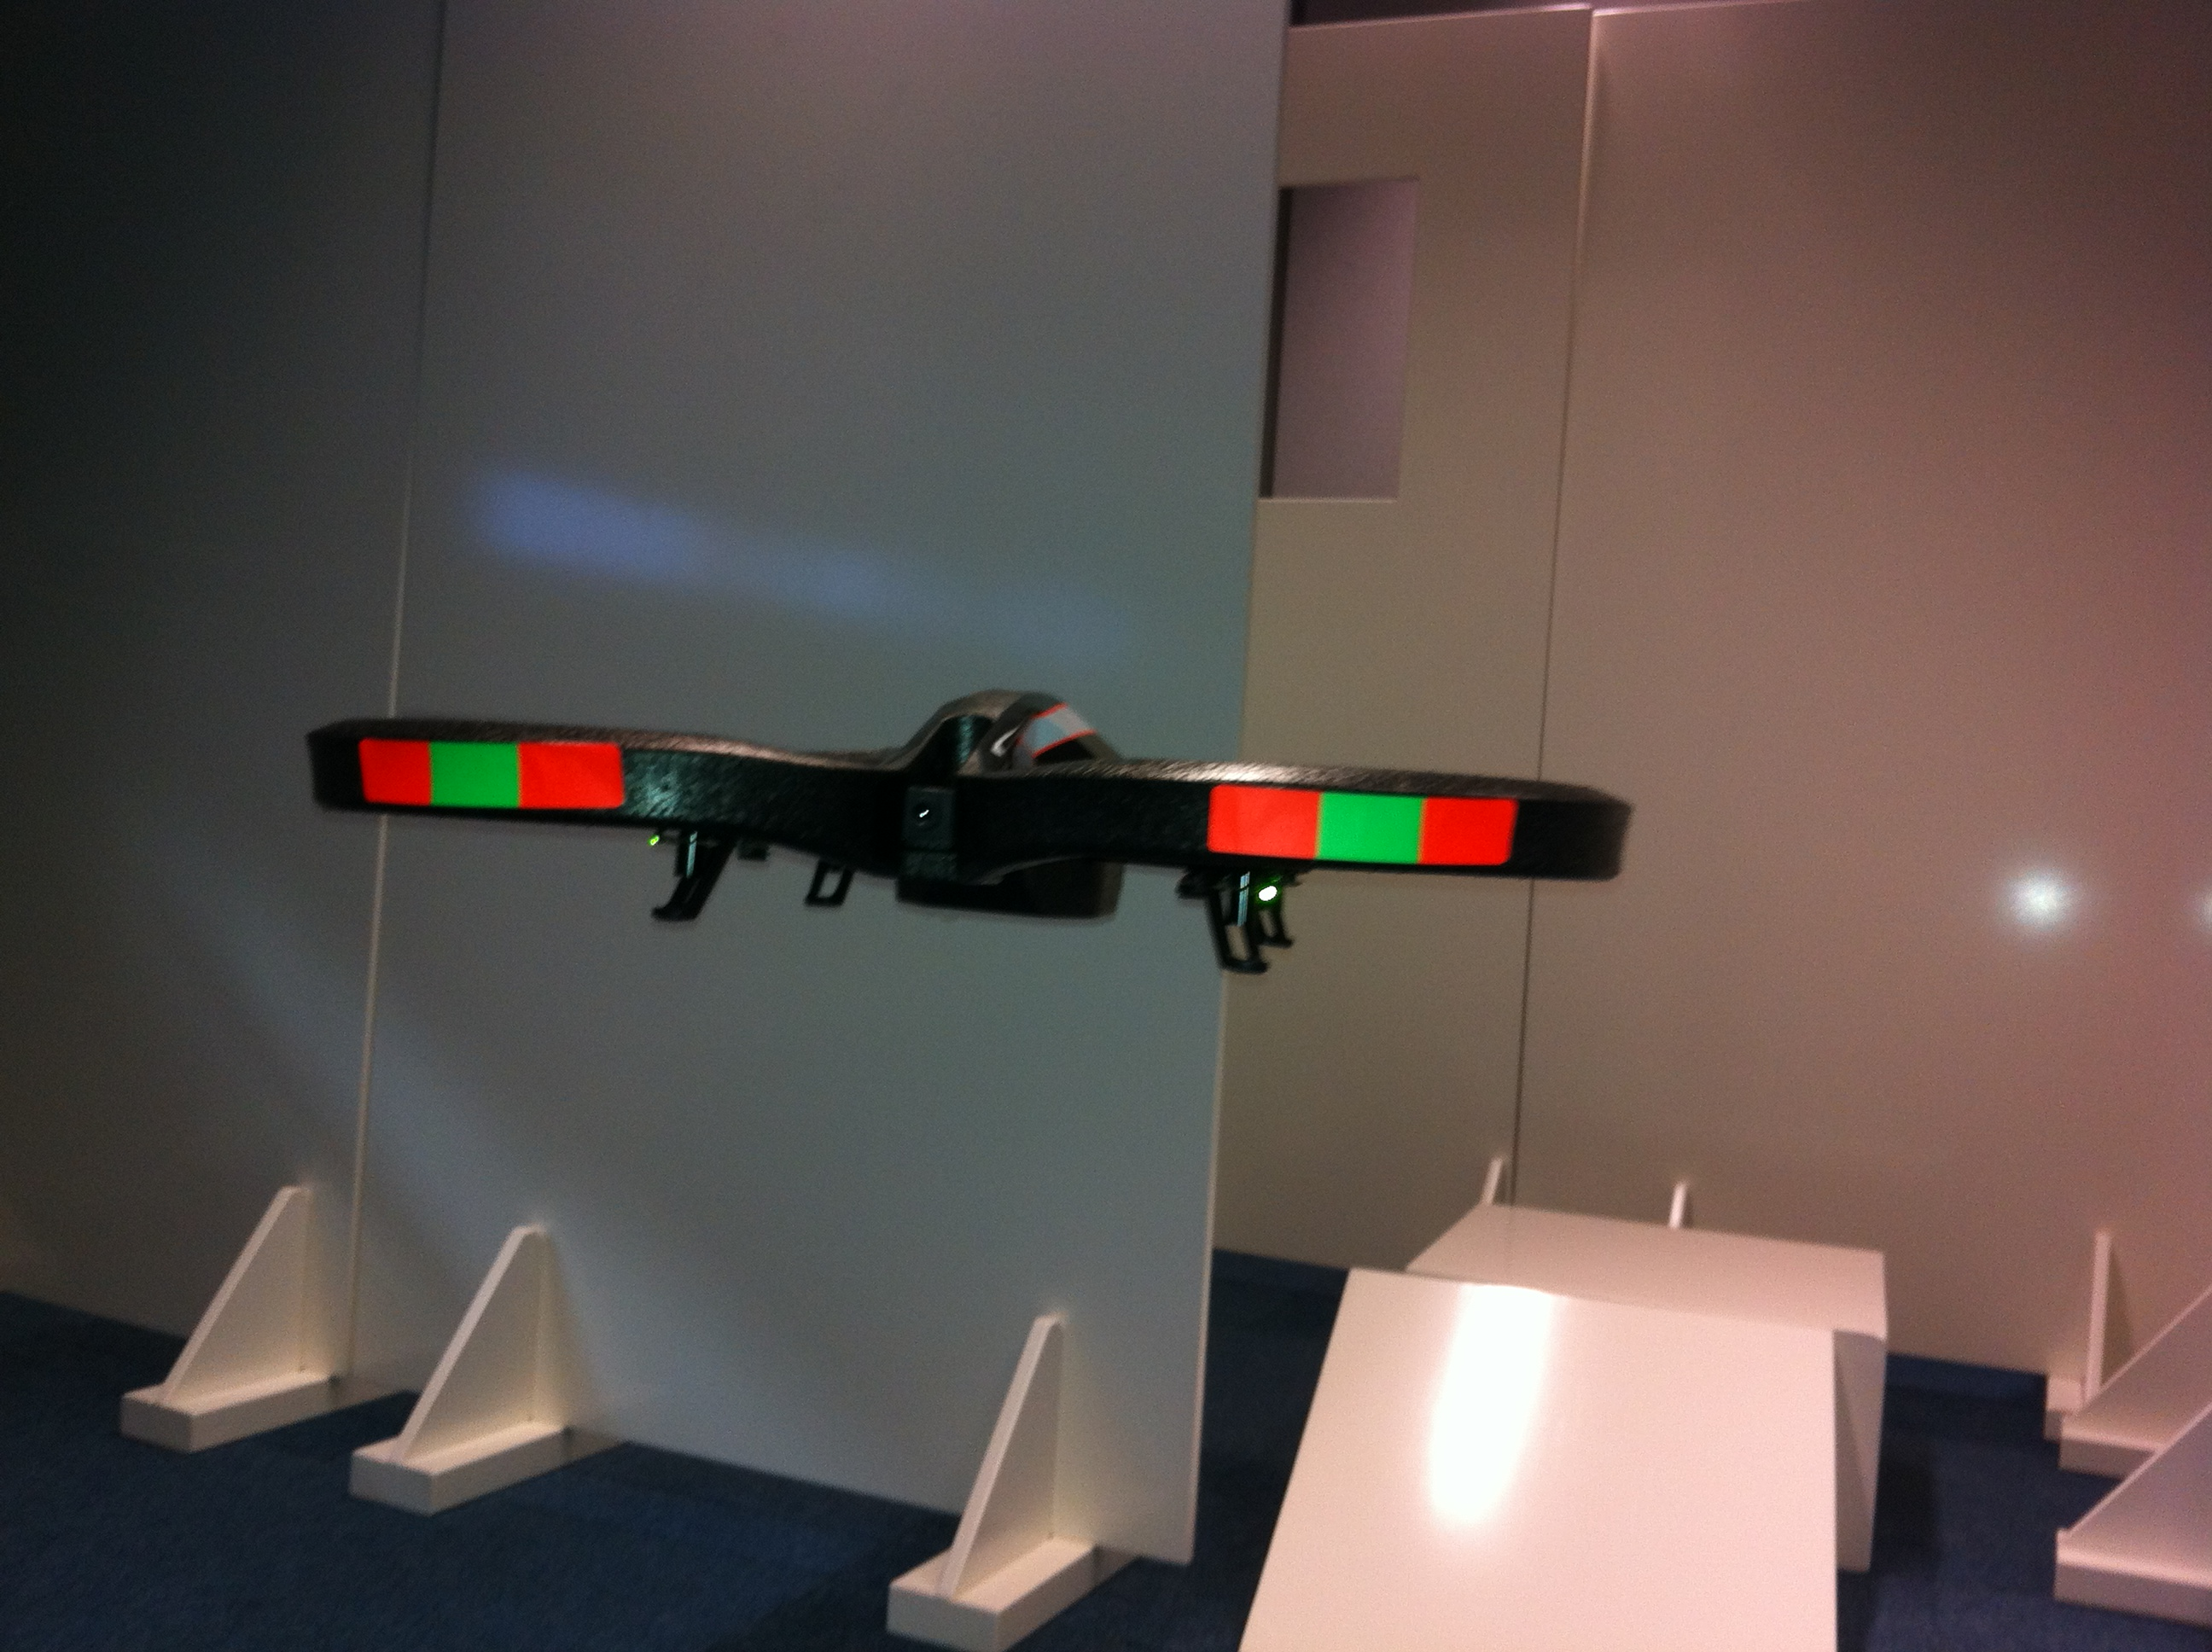
\includegraphics[width=0.7\textwidth]{images/title.jpg}\\\vspace{0.5cm}
\textbf{\textsc{A Bachelor Thesis by Camiel R. Verschoor}}
\end{center}
\end{frame}

\begin{frame}
  \titlepage
\end{frame}

\begin{frame}{Supervisors}
\begin{center}
\begin{tabular}{ c c }
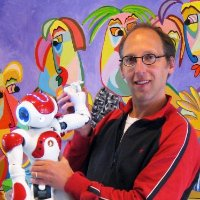
\includegraphics[width = 0.3\textwidth]{images/visser.jpg} & 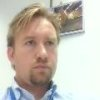
\includegraphics[width = 0.3\textwidth]{images/poppinga.jpg}\\
Dr. Arnoud Visser & Drs. Gerald Poppinga\\
Assistant Professor & R\&D Manager for mini UAS\\
University of Amsterdam & National Aerospace Lab (NLR)
\end{tabular}
\end{center}
\end{frame}

\begin{frame}{National Aerospace Lab NLR}
\begin{center}
\begin{tabular}{ c c }

\includegraphics[width = 0.3\textwidth]{images/nlr_logo.jpg} & 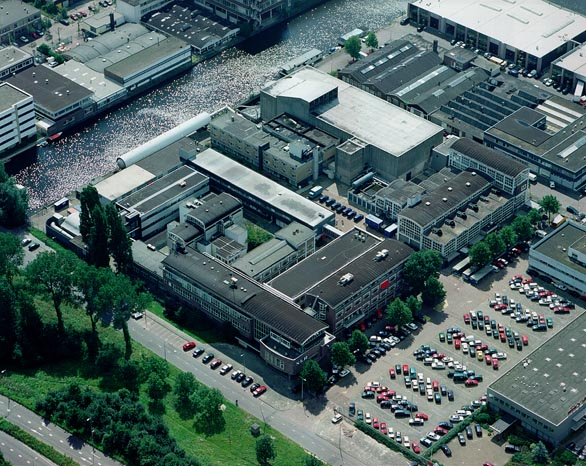
\includegraphics[width = 0.3\textwidth]{images/nlr_lucht.jpg}
\end{tabular}\\
NLR is the main knowledge enterprise in the Netherlands in the field of aviation and aerospace.
\end{center}
\end{frame}

\begin{frame}{Outline}
  \setcounter{tocdepth}{1}
  \tableofcontents
\end{frame}

\section{Introduction}
\subsection{Motivation}

\begin{frame}
\begin{block}{Motivation}
\begin{itemize}
\item Autonomous Robots require navigation.
\item GPS is unreliable in indoor and urban environments.
\item \textbf{Possible alternative:} vision-based line-following.
\end{itemize}
\end{block}
\begin{center}
\begin{tabular}{ c c }
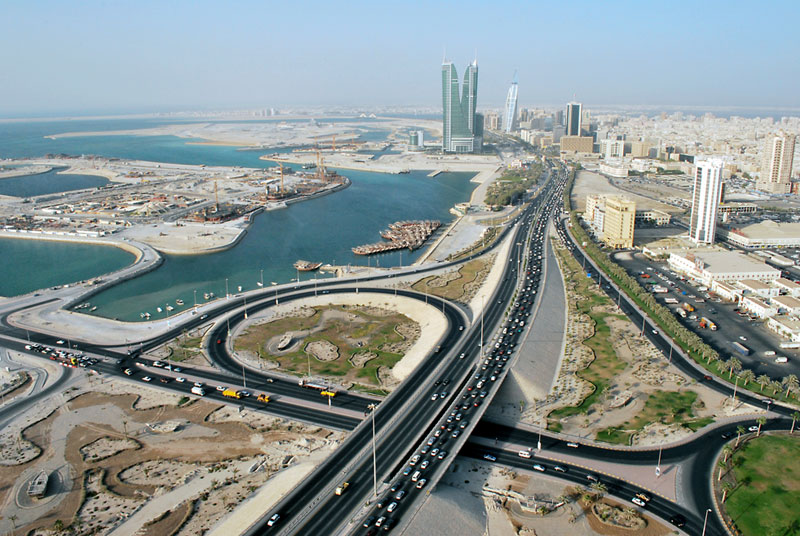
\includegraphics[width = 0.4\textwidth]{images/lucht_weg.jpg} & 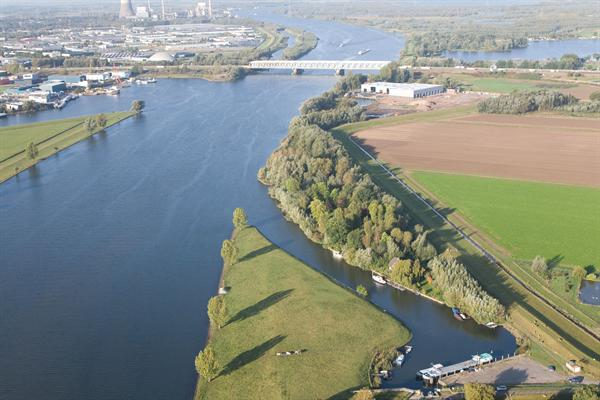
\includegraphics[width = 0.4\textwidth]{images/lucht_rivier.jpg}
\end{tabular}
\end{center}
\end{frame}

\begin{frame}
\begin{block}{Motivation}
\begin{itemize}
\item Various approaches of vision-based line-following.
\item Edge and motion detection suitable candidates \cite{Bills2011, Gerke2011}, but have weaknesses.
\item \textbf{Solution:} combine them to strengthen each others weaknesses.
\end{itemize}
\end{block}
\end{frame}

\subsection{Research Question}
\begin{frame}
\begin{block}{Research Question}
\begin{itemize}
\item To examine how edge and motion detection can be combined to strengthen each other in a line-following task.
\begin{itemize}
\item What is the optimal camera configuration?
\item What are the experimental settings that demonstrate the strength and weaknesses of these algorithms?
\item What is the performance and robustness of these vision-based methods to navigation?
\end{itemize}
\end{itemize}
\end{block}
\end{frame}

\subsection{Platform and Framework}
\begin{frame}
\begin{block}{Platform and Framework}
\begin{description}
\item[Platform] Parrot AR.Drone.
\begin{itemize}
\item Top and bottom camera.
\end{itemize}
\item[Framework] AR.Drone SLAM\footnote{\cite{Dijkshoorn2012}} a development framework.
\end{description}
\end{block}
\begin{center}
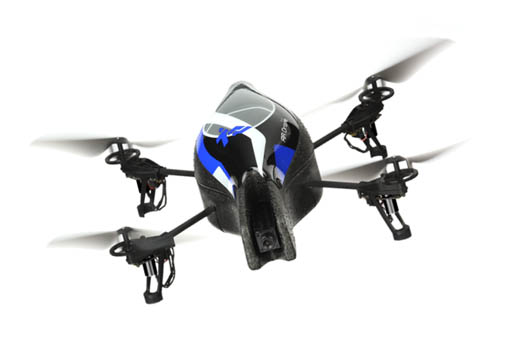
\includegraphics[width = 0.2\textwidth]{images/ardrone.jpg}
\end{center}
\end{frame}

\subsection{Related Work}
\begin{frame}
\begin{block}{Related Work}
\begin{itemize}
\item Corridor and Stair Following \cite{Bills2011}.
\item Power Line Detection \cite{Golightly2005, Zhengrong2008, Katrasnik2010}.
\item Obstacle Avoidance \cite{Jurriaans2011}.
\item Elementary Motion Detectors \cite{Gerke2011}.
\end{itemize}
\end{block}
\end{frame}

\begin{frame}
\begin{center}
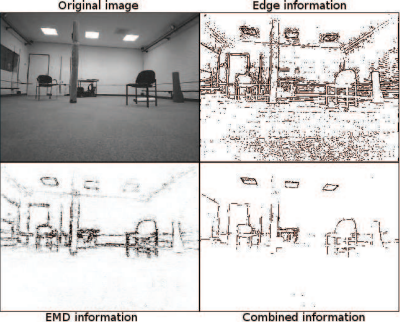
\includegraphics[width=0.7\textwidth]{images/gerke2011.png}
\footnote{\cite{Gerke2011}}
\end{center}
\end{frame}

\begin{frame}
\begin{block}{Related Work}
\begin{itemize}
\item Nearly all proposed methods use Hough Transform for feature extraction.
\item Edge and Motion detection have been suitable techniques for navigation .
\item Combination of Edge and Motion detection gave promising results.
\end{itemize}
\end{block}
\end{frame}

\section{Approach}
\subsection{Main Approach}
\begin{frame}
\begin{block}{Main Approach}
\xymatrix{Camera \ar[rrrr]_{Frame} & & & & Pre-processing \ar[dd]_{Binary\ image}\\
& & & &\\
World \ar[uu]_{Input} & & & & Feature\ extraction \ar[dd]_{Line\ segments}\\
& & & &\\
Flight\ controller \ar[uu]_{Flying} & & & & Navigation \ar[llll]_{Controls}}
\end{block}
\end{frame}

\begin{frame}
\begin{block}{Main Approach}
\begin{itemize}
\item Pre-processing. 
\begin{itemize}
\item Canny edge detector (Brightness changes).
\item Monocular stereo vision (Apparent motion).
\end{itemize}
\item Feature extraction.
\begin{itemize}
\item Probabilistic Hough Transform.
\end{itemize}
\item Navigation.
\end{itemize}
\end{block}
\end{frame}

\subsection{Pre-processing}
\begin{frame}
\begin{block}{Pre-processing}
\begin{itemize}
\item Canny edge detector (Brightness changes).
\item Monocular stereo vision (Apparent motion).
\end{itemize}
\end{block}
\end{frame}

\begin{frame}
\begin{block}{Edge detection}
\begin{itemize}
\item Colour filter.
\item Gaussian Smoothing (Removes noise).
\item Canny edge detector (Brightness changes).
\end{itemize}
\end{block}
\begin{block}{Result}
Binary image.
\end{block}
\end{frame}

\begin{frame}
\begin{block}{Edge detection}
\begin{center}
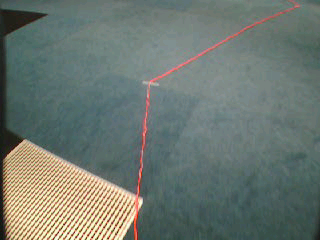
\includegraphics[width=0.3\textwidth]{images/canny_image.png}
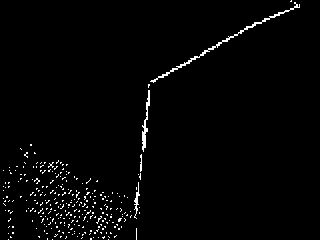
\includegraphics[width=0.3\textwidth]{images/canny_image_filter.png}\\
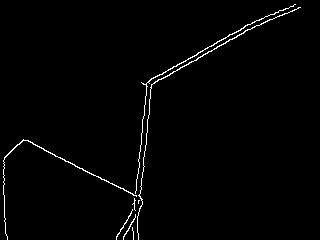
\includegraphics[width=0.3\textwidth]{images/canny_detector.png}
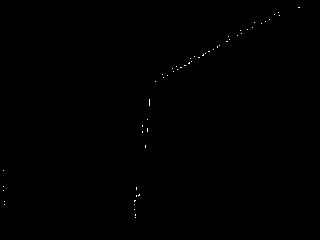
\includegraphics[width=0.3\textwidth]{images/canny_combine.png}
\end{center}
\end{block}
\end{frame}

\begin{frame}
\begin{block}{Monocular Stereo Vision}
\begin{center}
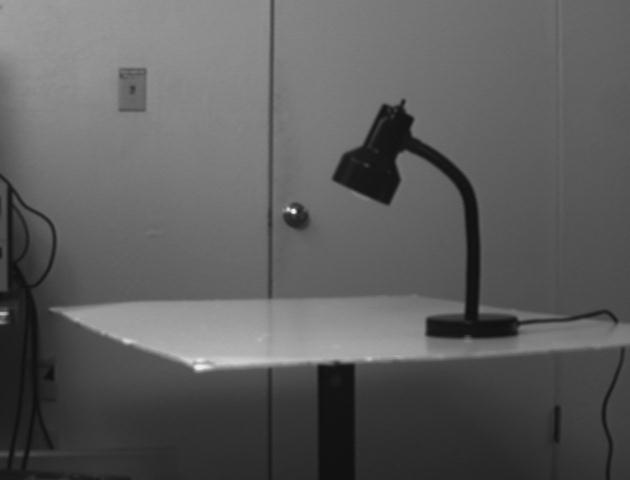
\includegraphics[width=0.3\textwidth]{images/lamp_left.jpg}
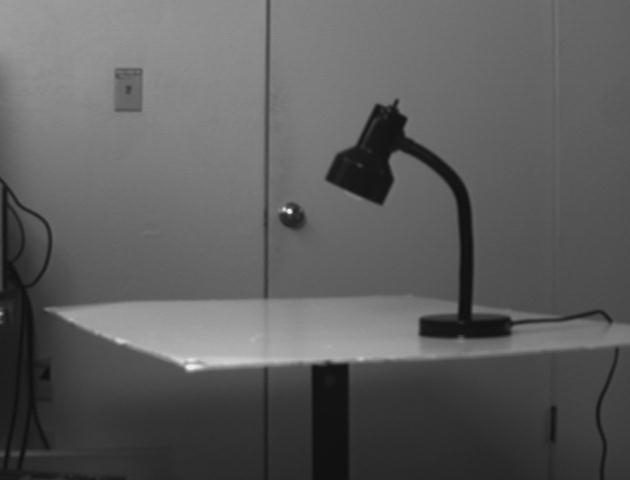
\includegraphics[width=0.3\textwidth]{images/lamp_right.jpg}
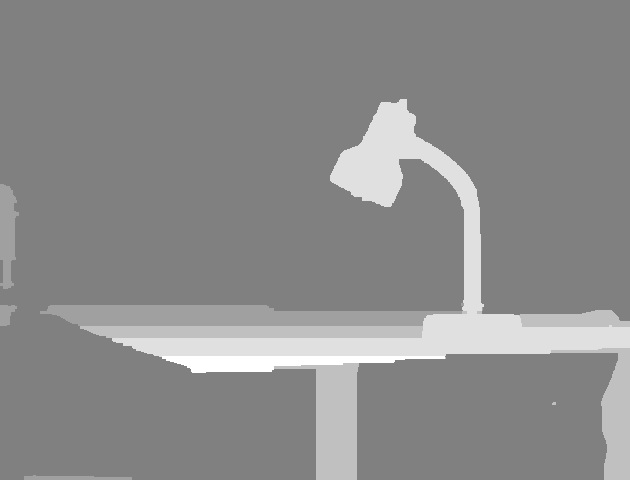
\includegraphics[width=0.3\textwidth]{images/lamp_disparity.jpg}
\end{center}
\end{block}
\end{frame}


\begin{frame}
\begin{block}{Monocular Stereo Vision}
\begin{itemize}
\item Find features \cite{Shi1994}.
\item Optical Flow.
\item Determining fundamental matrix (mapping between frames).
\item Rectify images.
\item Stereo matching.
\item Thresholding.
\end{itemize}
\end{block}
\begin{block}{Result}
Binary image
\end{block}
\end{frame}

\begin{frame}
\begin{block}{Optical Flow}
\begin{center}
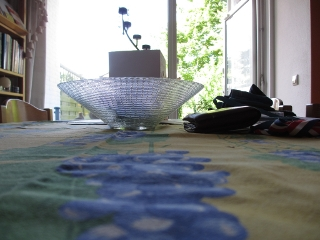
\includegraphics[width=0.3\textwidth]{images/frame0.jpg}
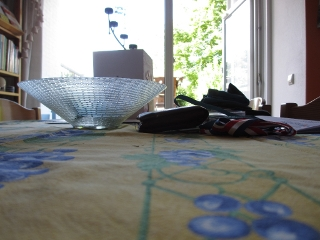
\includegraphics[width=0.3\textwidth]{images/frame1.jpg}
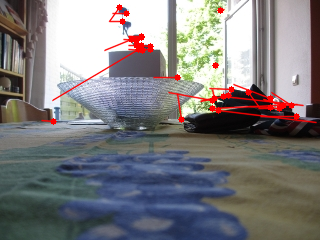
\includegraphics[width=0.3\textwidth]{images/optical_flow.png}
\end{center}
\end{block}
\end{frame}

\begin{frame}
\begin{block}{Monocular Stereo Vision}
\begin{center}
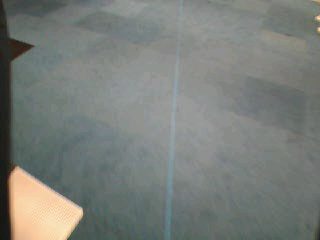
\includegraphics[width=0.3\textwidth]{images/stereo_image.png}
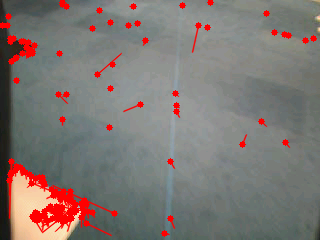
\includegraphics[width=0.3\textwidth]{images/stereo_optical_flow.png}
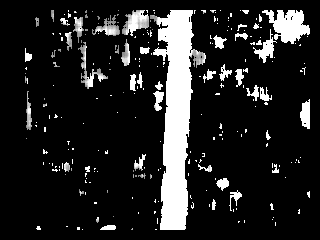
\includegraphics[width=0.3\textwidth]{images/stereo_disparity.png}\\
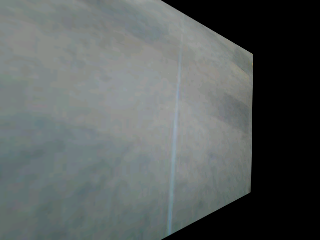
\includegraphics[width=0.3\textwidth]{images/stereo_left.png}
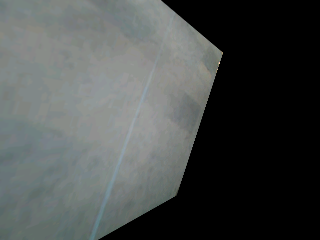
\includegraphics[width=0.3\textwidth]{images/stereo_right.png}
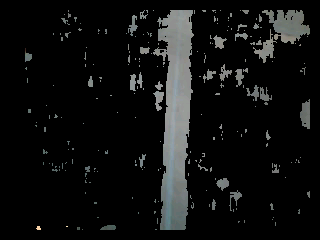
\includegraphics[width=0.3\textwidth]{images/stereo_disparity_cut.png}
\end{center}
\end{block}
\end{frame}

\subsection{Feature extraction}
\begin{frame}
\begin{block}{Feature extraction}
\begin{itemize}
\item Probabilistic Hough Transform \cite{Kiryati1991}.
\begin{itemize}
\item Grouping points of parametrized image objects.
\item Voting procedure.
\item Takes only subset of the found points.
\end{itemize}
\end{itemize}
\end{block}
\end{frame}

\begin{frame}
\begin{block}{Probabilistic Hough Transform}
\begin{center}
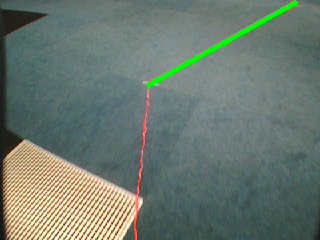
\includegraphics[width=0.3\textwidth]{images/canny_PHT.png}
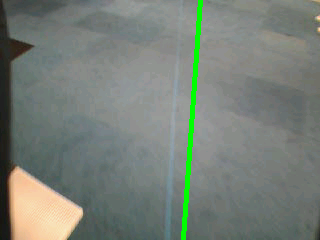
\includegraphics[width=0.3\textwidth]{images/stereo_PHT.png}
\end{center}
\end{block}
\end{frame}

\subsection{Navigation}
\begin{frame}
\begin{block}{Navigation}
\begin{itemize}
\item Fly towards line.
\item Fly over it.
\end{itemize}
\end{block}
\end{frame}

\section{Experiments}
\subsection{Camera Configuration}
\begin{frame}
\begin{block}{Camera Configuration}
\begin{center}
\begin{tabular}{c c}
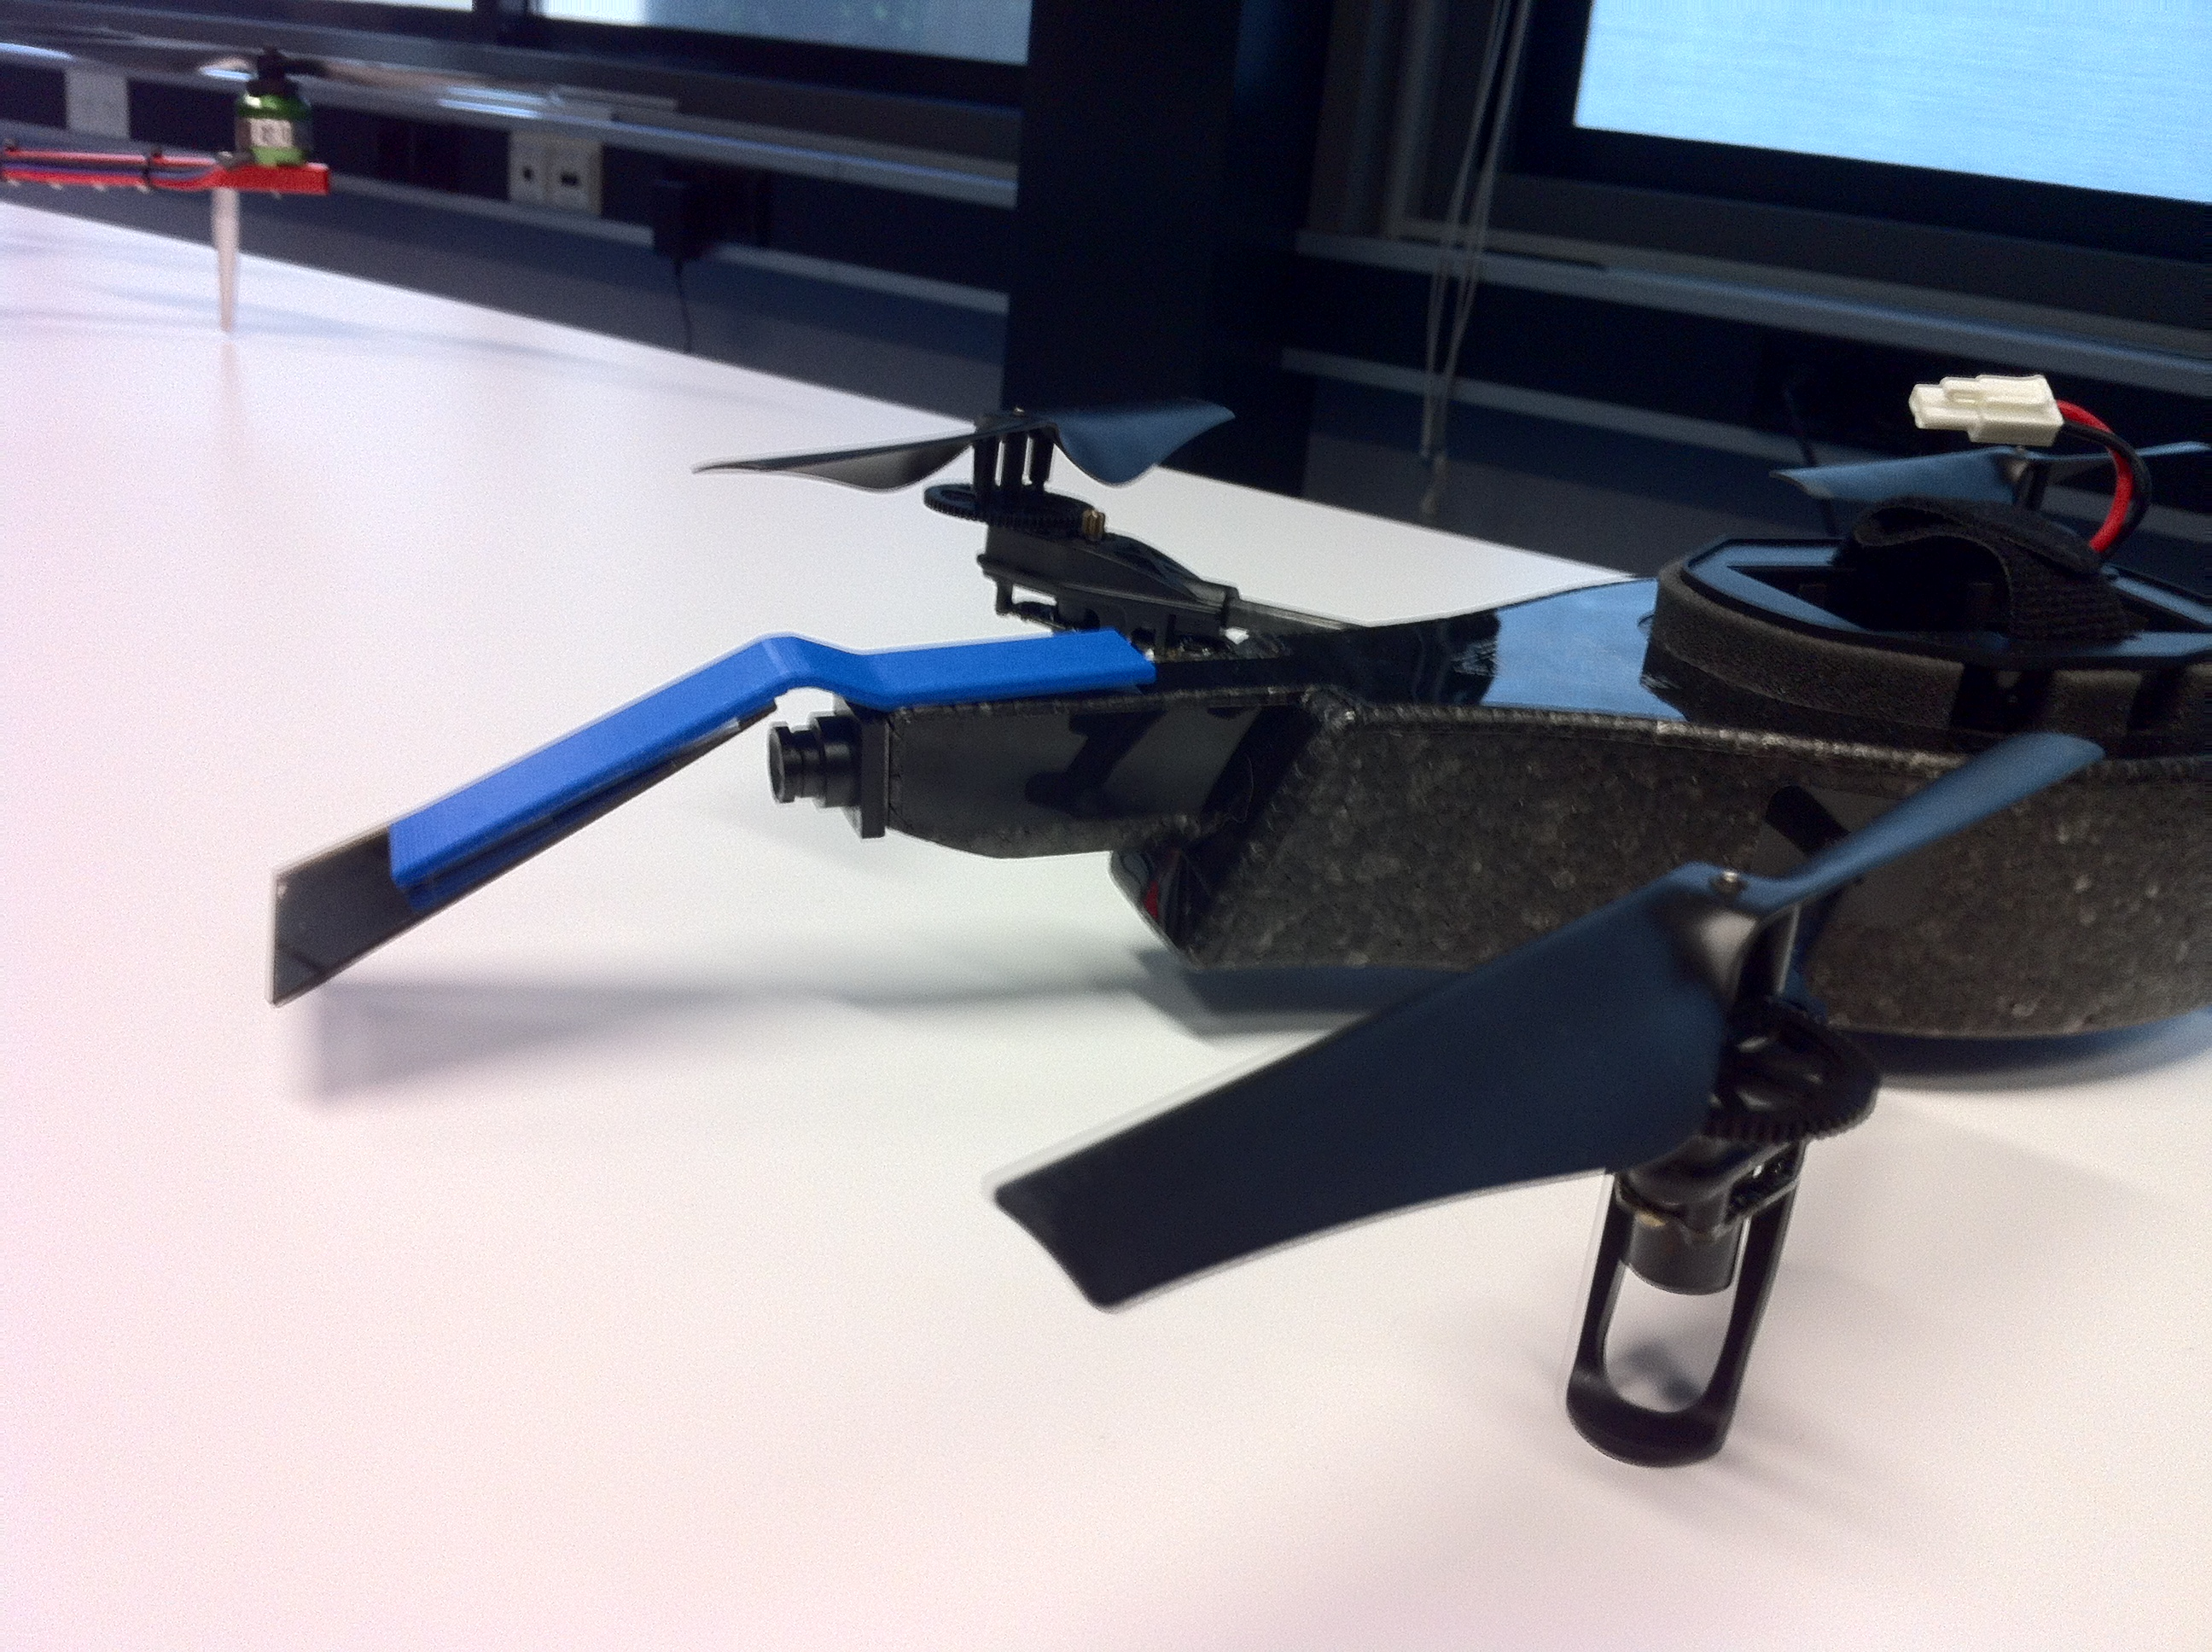
\includegraphics[width = 0.3\textwidth]{images/ardrone_mirror.jpg} & 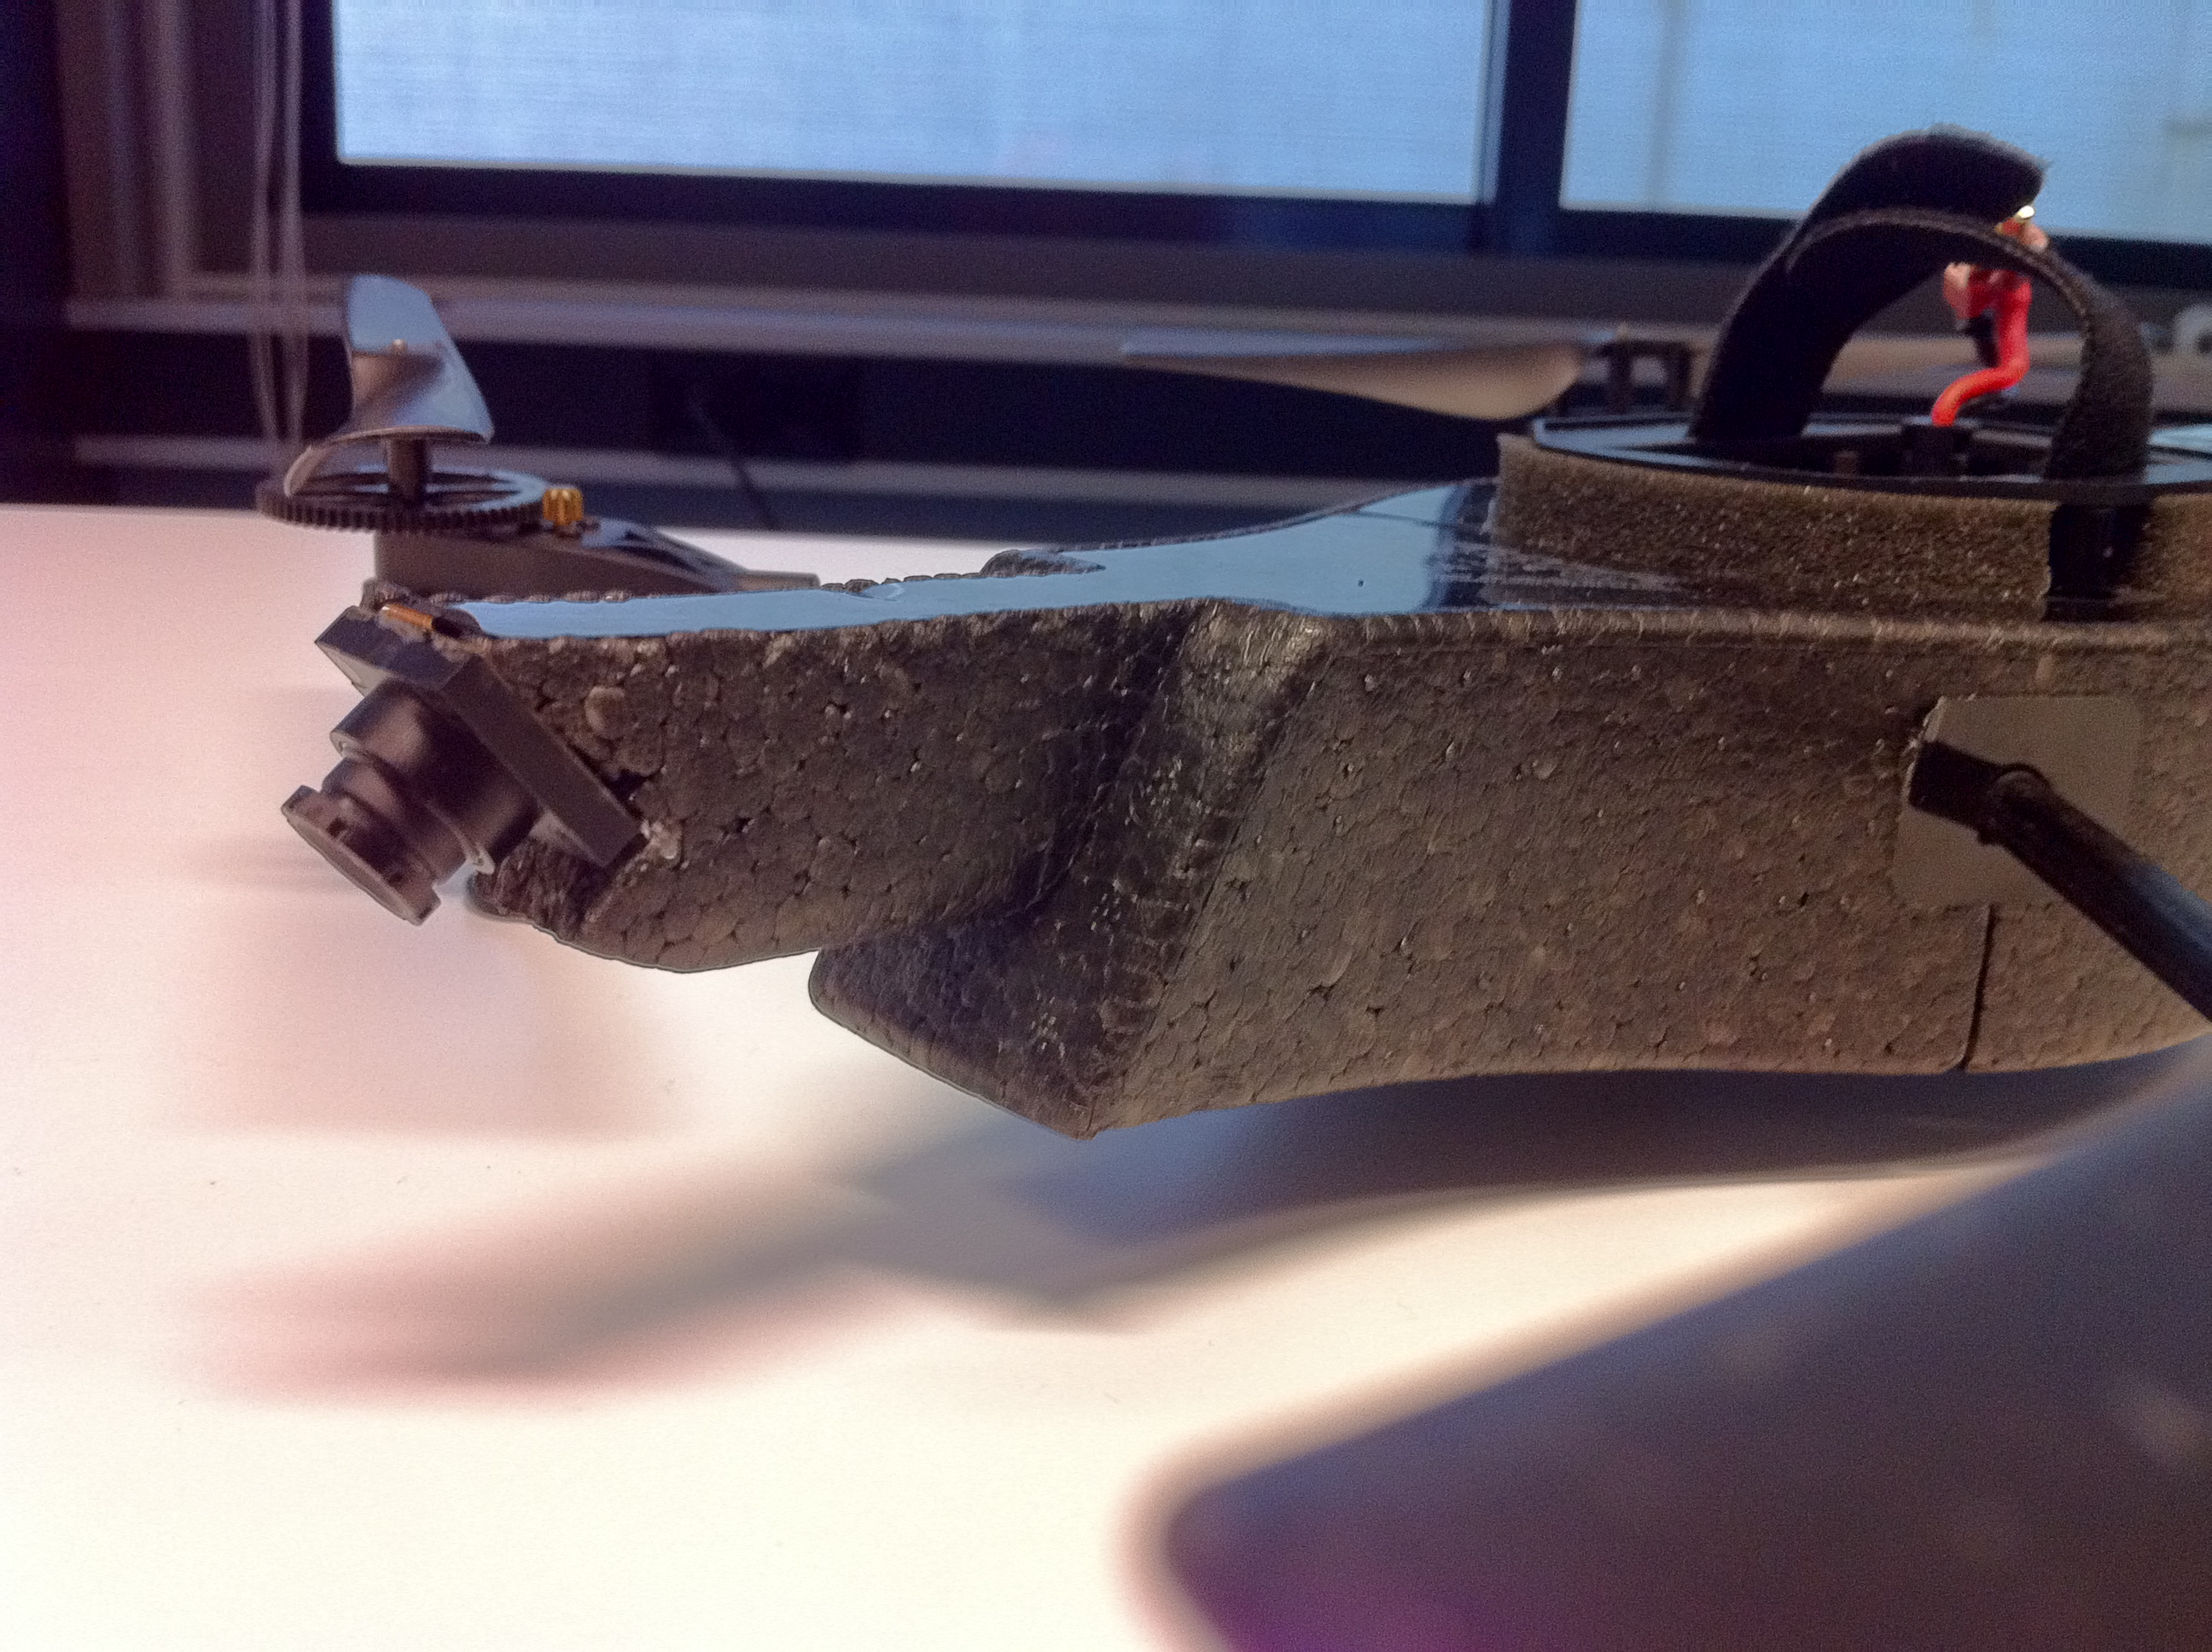
\includegraphics[width = 0.3\textwidth]{images/ardrone_modification.jpg}
\end{tabular}
\end{center}
\end{block}
\end{frame}

\subsection{Experiments}
\begin{frame}
\begin{block}{Experiments}
\begin{center}
\begin{tabular}{c c}
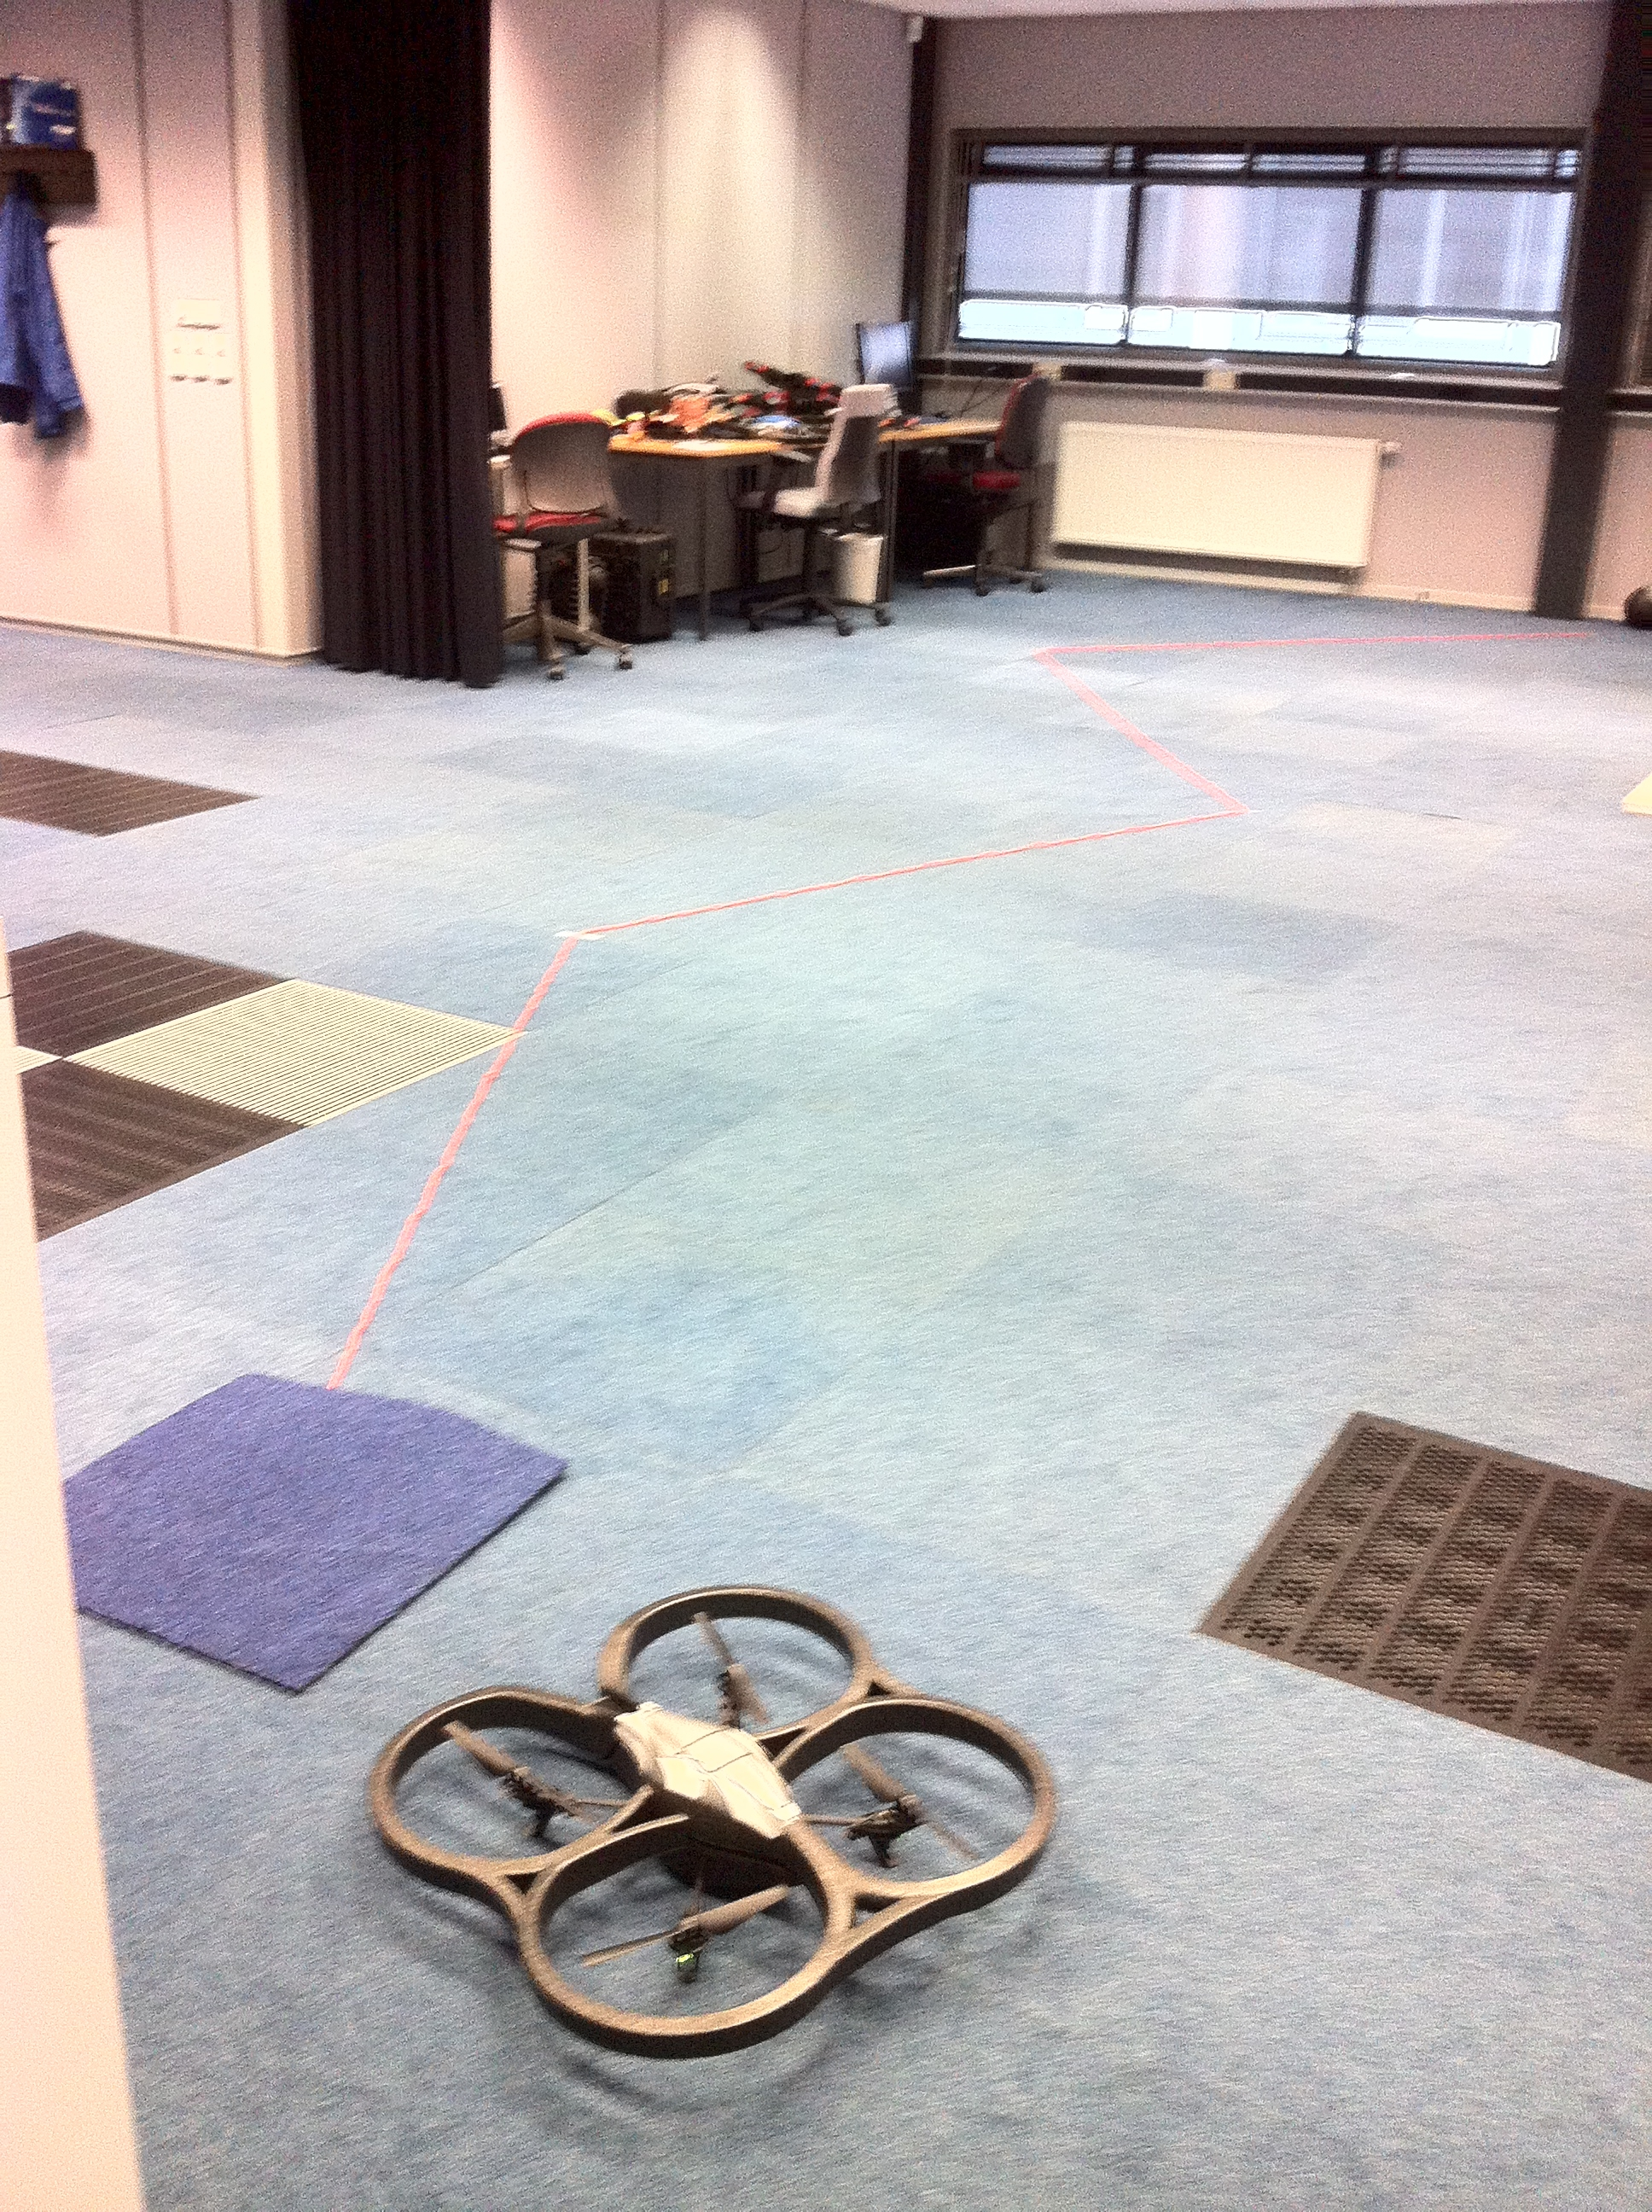
\includegraphics[width = 0.3\textwidth]{images/experiment1.jpg} & 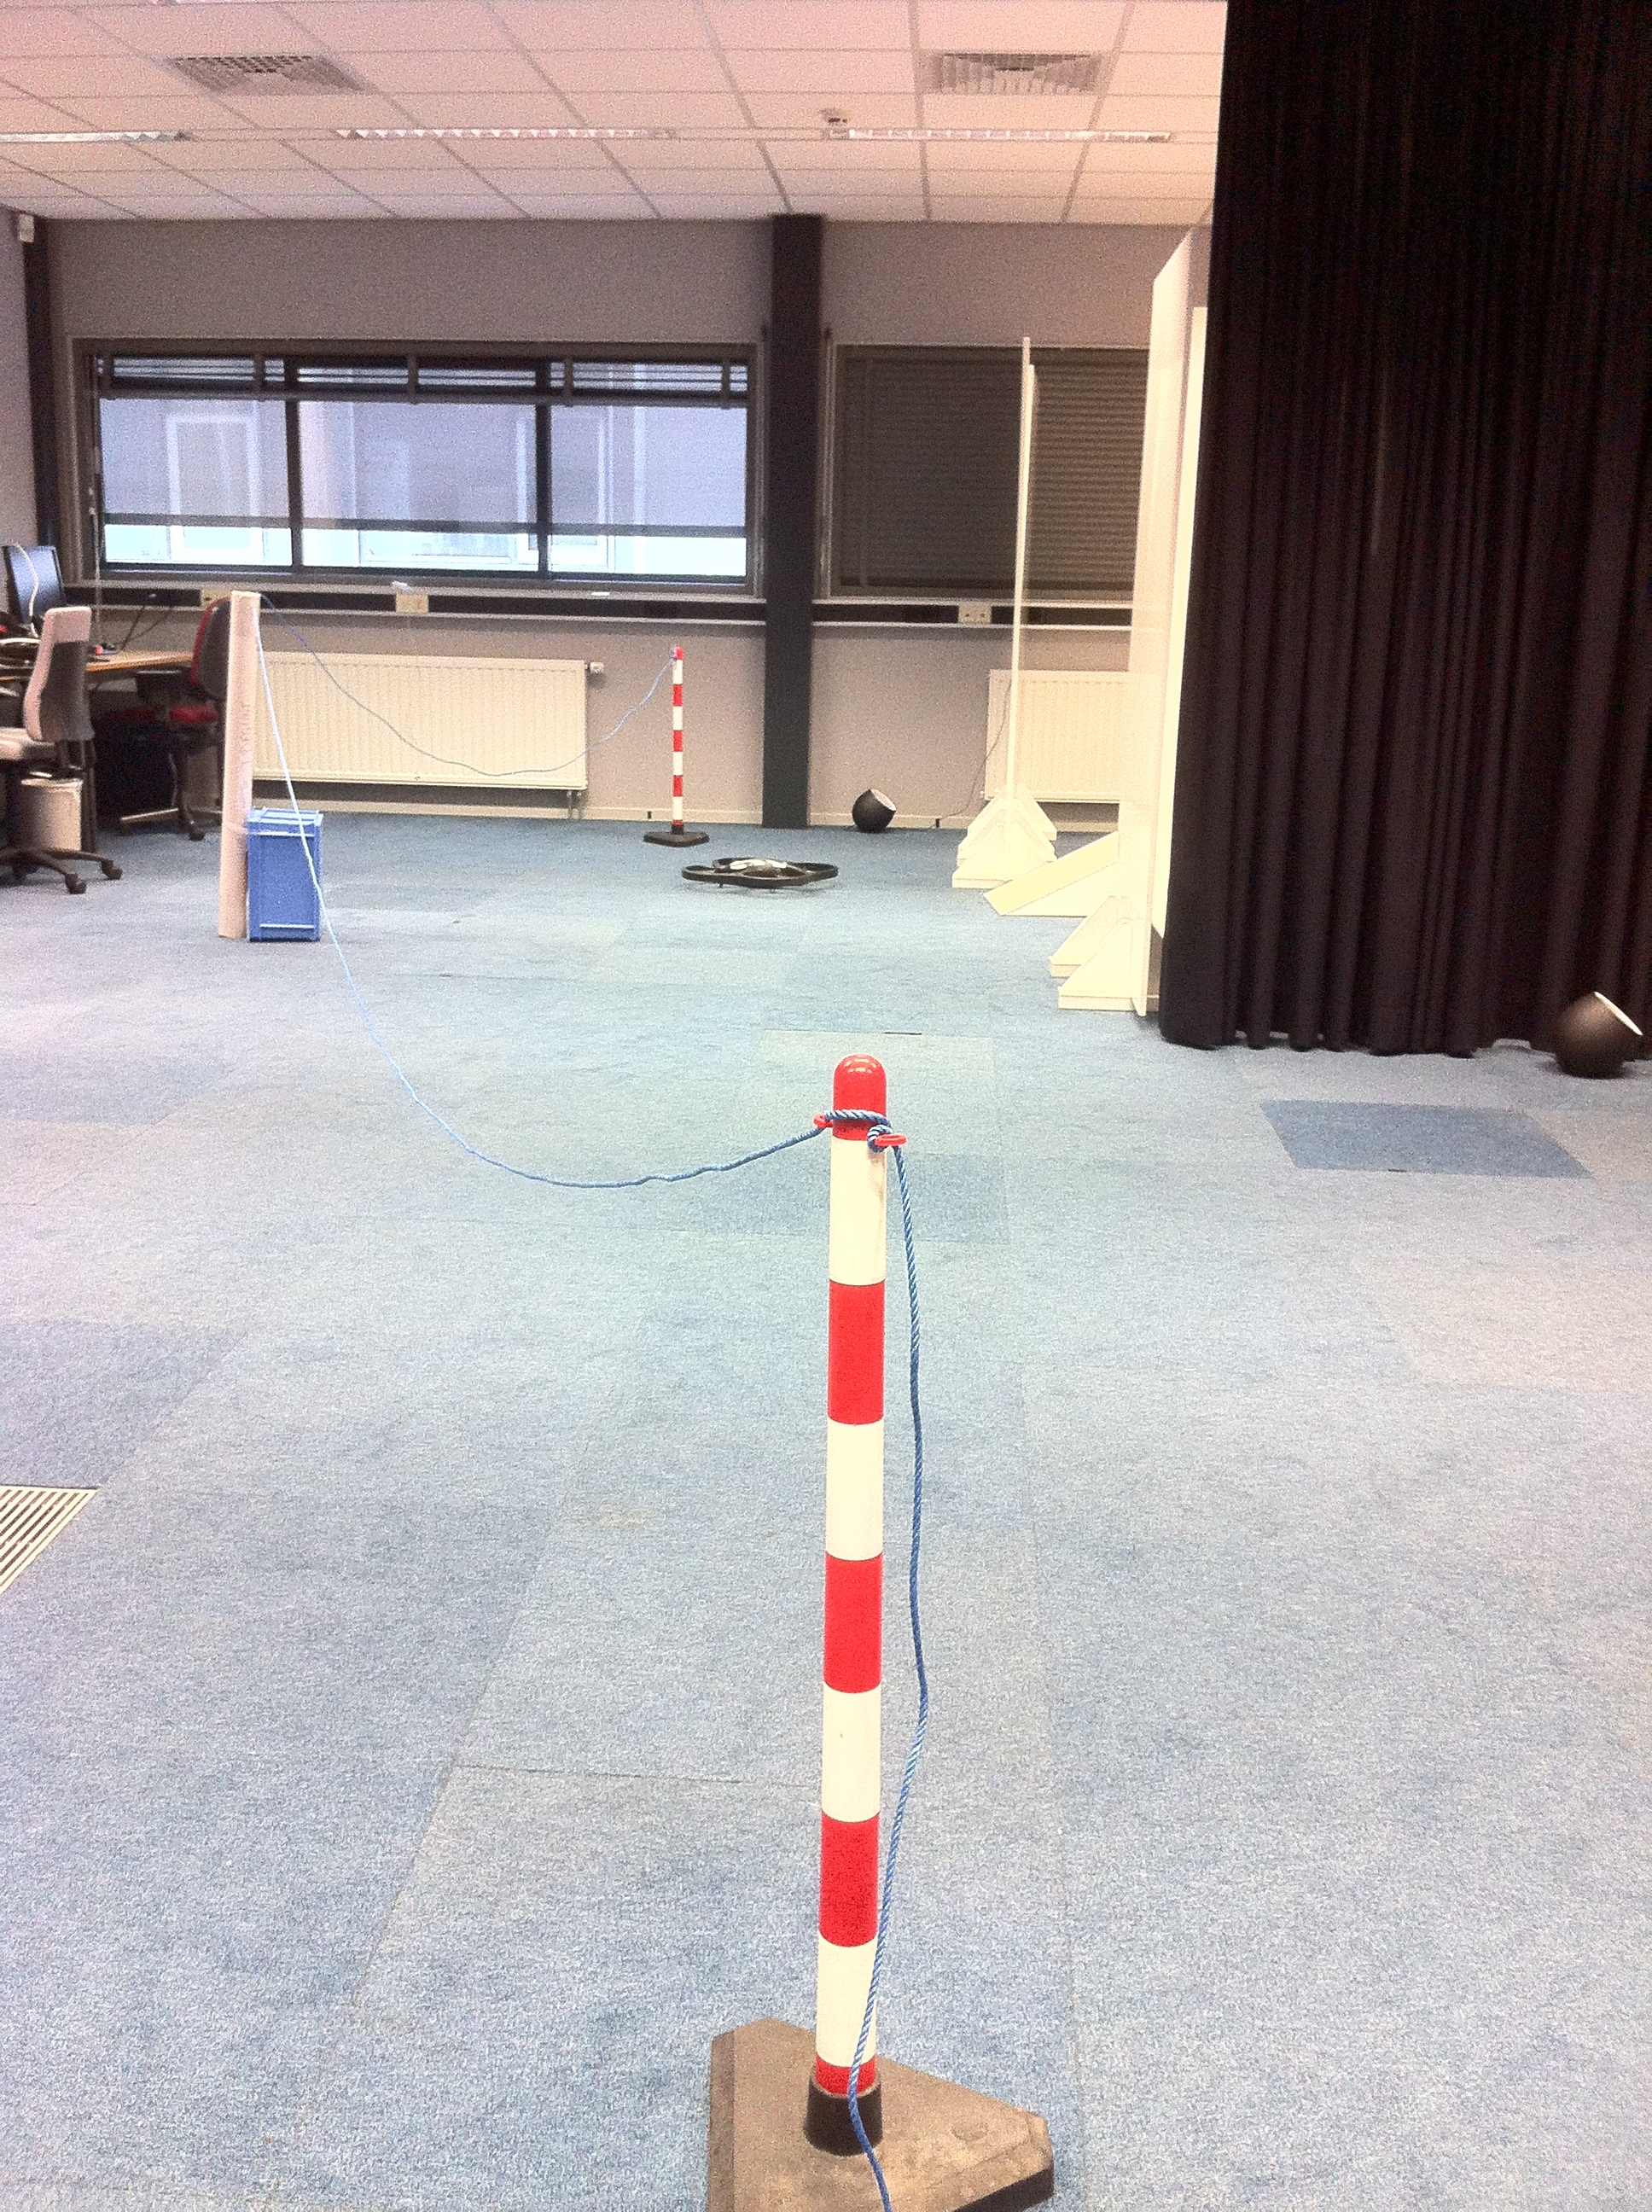
\includegraphics[width = 0.3\textwidth]{images/experiment2.jpg}
\end{tabular}
\end{center}
\end{block}
\end{frame}

\subsection{Evaluation Criteria}
\begin{frame}
\begin{block}{Evaluation Criteria}
\begin{itemize}
\item Detection of line.
\item Direction of line.
\end{itemize}
\end{block}
\end{frame}

\section{Results}
\subsection{Camera Configuration}
\begin{frame}
\begin{block}{Camera Configuration}
\begin{block}{Mirror Construction}
\begin{itemize}
\item Distorted images.
\item No optimal angle.
\end{itemize}
\end{block}

\begin{block}{Modification}
\begin{itemize}
\item Sharp images.
\item Optimal angle.
\end{itemize}
\end{block}
\end{block}
\end{frame}
\subsection{Experiments}
\begin{frame}
\begin{block}{Experiment 1}
\textbf{Edge detection}\\\vspace{0.1cm}
\begin{tabular}{| l | l | l |}
\hline
\textbf{Performance} & True & False\\
\hline
Detected  & 528 (97.8\%) & 12 (2.2\%)\\
\hline
Direction & 503 (93.1\%) & 37 (6.9\%)\\
\hline
\end{tabular}\\\vspace{0.1cm}

\textbf{Motion Detection}\vspace{0.1cm}

\begin{tabular}{| l | l | l |}
\hline
\textbf{Performance} & True & False\\
\hline
Detected  & 53 (9.8\%) & 487 (90.2\%)\\
\hline
Direction & 37 (6.9\%) & 503 (93.1\%)\\
\hline
\end{tabular}
\end{block}
\end{frame}

\begin{frame}
\begin{block}{Conclusion Experiment 1}
\begin{itemize}
\item Shows the strength of edge detection.
\item Shows the weakness of motion detection.
\item Edge detection can strengthen motion detection.
\end{itemize}
\end{block}
\end{frame}

\begin{frame}
\begin{block}{Experiment 2}
\textbf{Edge Detection}\\\vspace{0.1cm}

\begin{tabular}{| l | l | l |}
\hline
\textbf{Performance} & True & False\\
\hline
Detected  & 69 (29.0\%) & 169 (71.0\%)\\
\hline
Direction & 58 (24.4\%) & 180 (85.6\%) \\
\hline
\end{tabular}\\\vspace{0.1cm}

\textbf{Motion Detection}\\\vspace{0.1cm}

\begin{tabular}{| l | l | l |}
\hline
\textbf{Performance} & True & False\\
\hline
Detected  & 96 (40.3\%) & 142 (59.7\%)\\
\hline
Direction & 87 (36.6\%) & 137 (63.4\%) \\
\hline
\end{tabular}
\end{block}

\end{frame}

\begin{frame}
\begin{block}{Conclusion Experiment 2}
\begin{itemize}
\item Shows the weakness of edge detection.
\item Motion detection worked suboptimal\\\textbf{Possible solutions}
\begin{itemize}
\item Look at average motion.
\item Other datasets.
\item Other algorithms, Elementary Motion Detectors \cite{Gerke2011}.
\end{itemize}
\end{itemize}
\end{block}
\end{frame}

\begin{frame}{}
\begin{block}{Video}
\begin{itemize}
\item \href{http://youtu.be/MmxhRnjHIv4}{AR.Drone follows line.}
\item \href{http://youtu.be/cSdcYHPiah4}{Monocular Stereo Vision}
\end{itemize}

\end{block}
\end{frame}


\section{Conclusion}
\begin{frame}
\begin{block}{Conclusion}
\begin{itemize}
\item \textbf{Camera configuration:} Modification was the most optimal solution.
\item \textbf{Experimental settings:} Contrasting line on the ground and low contrast line in the air.
\item \textbf{Performance and robustness:}  Algorithms can strengthen each other, improvements can be made.
\end{itemize}
\end{block}
\end{frame}



\section{Questions}
\begin{frame}{Questions?}
\begin{center}
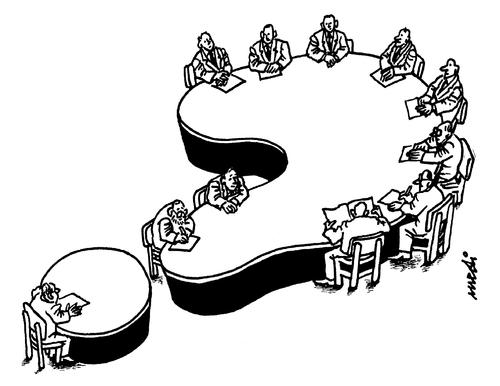
\includegraphics[width = 0.7\textwidth]{images/questions.jpg}
\end{center}
\end{frame}

\begin{frame}{Acknowledgements}
\begin{block}{I would like to thank for their guidance and support
:}
\begin{itemize}
\item Arnoud Visser
\item Gerald Poppinga
\end{itemize}
\end{block}
\end{frame}

\section{Relevant Literature}
\begin{frame}{}
\begin{block}{Relevant videos}
\begin{itemize}
\item \href{http://youtu.be/7XyddRwP_KA}{Corridor following}
\item \href{http://youtu.be/MF0nHhMKl5g}{Various tasks}
\end{itemize}

\end{block}
\end{frame}


\begin{frame}[allowframebreaks]{Relevant Literature}
\footnotesize
\bibliographystyle{apalike}
\bibliography{references}
\end{frame}

\end{document}
